\documentclass[10pt,a4paper]{amsart}
\usepackage[margin=19mm]{geometry}
\usepackage{amsmath,amssymb,mathtools}
\usepackage[scr=rsfs,cal=euler]{mathalfa}
\usepackage{xfrac}
\usepackage[unicode,hidelinks,bookmarks=false]{hyperref}
\newcommand{\ie}{i.e.\ }
\newcommand{\cf}{cf.\ }
\newcommand{\resp}{respectively\ }
\newcommand{\Subsection}{\subsection}
\providecommand{\nobreakdash}{\nobreak\hbox{-}}
\setlength{\emergencystretch}{2em}
\multlinegap0pt
\usepackage{tikz}
\usepackage{amssymb}
\usepackage{float}
\newtheorem{thm}{Theorem}
\newtheorem{scope}{Scope}
\usepackage{cleveref}
\crefname{thm}{Theorem}{Theorems}
\crefname{scope}{Scope}{Scopes}
\newcommand{\edmonds}{{\textsc{Greedy Edmonds}}}
\newcommand{\opt}{{\mathsf{OPT}}}
\title{Cluster deletion in cographs, permutation graphs, and graphs with bounded clique number}
\author{Nicola Galesi, Tony Huynh, Arnaud Patey, Fariba Ranjbar}
\date{Source: arXiv:2505.00922v4 (CC BY 4.0)}
\begin{document}
\maketitle

\noindent\emph{Source and licence.} Cluster deletion in cographs, permutation graphs, and graphs with bounded clique number. Version arXiv:2505.00922v4 (CC BY 4.0), distributed by arXiv under the Creative Commons Attribution 4.0 International licence, http://creativecommons.org/licenses/by/4.0/, as recorded in the arXiv licence metadata for this exact version and shown on the abstract page https://arxiv.org/abs/2505.00922v4. Full licence notice: \texttt{licenses/arxiv-2505.00922-CC-BY-4.0.txt}.\par\smallskip

\noindent\textit{Editorial scope.} Counted unit: the article's thm thm:tight (source0.tex lines 1324--1337). The article's complete original proof of it is delivered with it (source0.tex lines 1339--1604, one \texttt{proof} environment of 266 lines). No mathematics is written, repaired or re-derived: the statement and the proof are the article's own lines, in the article's own notation, and no retained line is substituted or re-flowed.  No further source-local context is needed: every cross-reference of every retained line resolves inside the two delivered spans.  Nothing was omitted from any retained span, so the package carries no omission record.  No retained line contains a citation, so the wrapper carries no bibliography and no bibliography entry.  The retained lines contain the article's own diagram code, which the wrapper typesets with the standard tikz packages; no image file is delivered and the package declares no asset dependency.  Editorial formatting only, in addition: an AMS \texttt{amsart} preamble that restates the article's own declarations and macros used by the retained lines, namely the environments \texttt{thm}, \texttt{scope} on separate counters, together with the standard packages those lines need.  The retained environments print in this document as Theorem 1, Scope 1 in order of appearance, whereas the article prints the same items with the numbering of its own full document.  The complete native source of the article as distributed in the arXiv e-print for this exact version is bundled unchanged as \texttt{sources/177458/source0.tex}.
\begin{thm} \label{thm:tight}
For every integer $\ell\geq 3$, there are infinitely many graphs $G$
with $\omega(G)=\ell$ and clique partitions $\mathcal{X}$ that can
be output by \edmonds{} such that
\[
   \opt=
   \frac{2\binom{\ell}{2}}{\binom{\ell}{2}+1}
   |E(\mathcal{X})|
   \qquad\text{and}\qquad
   |E(\overline{\mathcal{X}})| = 2\,\opt_{\mathrm{CD}},
\]
where $\opt$ is the maximum number of edges in a clique partition of
$G$, and $\opt_{\mathrm{CD}}=|E(G)|-\opt$ is the minimum number of edges whose deletion turns $G$ into a cluster graph.
\end{thm}

\begin{proof}
Fix $\ell\geq 3$, let
$L=\operatorname{lcm}(3,4,\ldots,\ell)$, and let $m$ be any positive
multiple of $L$. Begin with $m$ pairwise disjoint
\emph{row sets} $R_1,\ldots,R_m$, each containing $\ell$ vertices.
We recursively define disjoint sets $C_1,C_2,\ldots,C_t$. Put
$N_0=m\ell$. As long as
\[
   k_i:=\left\lceil\frac{N_{i-1}}{m}\right\rceil\geq 3,
\]
choose $C_i$ to consist of $k_i$ vertices in distinct rows and put
$N_i=N_{i-1}-k_i$. Choose these vertices from the $k_i$ largest current rows, breaking ties so that, after deleting
$C_1\cup\cdots\cup C_i$, the numbers of remaining vertices in the
rows differ by at most one (this is possible since $k_i\leq\ell
\leq m$). Let $t$ be the last index produced by this procedure.

Define $G_{\ell,m}$ on the $m\ell$ vertices by making every row
$R_j$ a clique, making every $C_i$ a clique, and adding no other
edges. See~\Cref{fig:G6} for a depiction of $G_{6,6}$.

        

\begin{figure} 
$$
    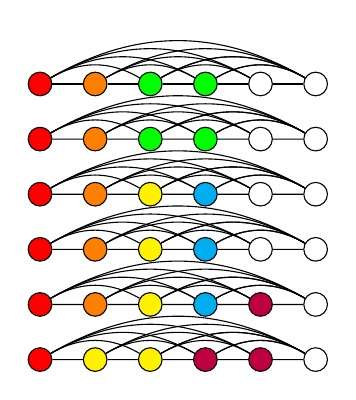
\begin{tikzpicture}[scale = 0.7]
    \tikzstyle{vertex}=[circle, draw=black, inner sep=0.cm, minimum size=3mm]
	\begin{scope}
	   %%% FIRST ROW %%%%%%
		\node[vertex,fill=red] (11) at (-1,-2){};
		\node[vertex,fill=orange] (12) at (0,-2){};
		\node[vertex,fill=green] (13) at (1,-2){};
		\node[vertex,fill=green] (14) at (2,-2){};
		\node[vertex] (15) at (3,-2){};
		\node[vertex] (16) at (4,-2){};
		\draw[-] (11) -- (12) node [midway,above] {};
		\draw[-] (12) -- (13) node [midway,above] {};
		\draw[-] (13) -- (14) node [midway,above] {};
		\draw[-] (14) -- (15) node [midway,above] {};
		\draw[-] (15) -- (16) node [midway,above] {};
		\draw[-] (11) to [bend left] (16);
        \draw[-] (11) to [bend left] (15);
		\draw[-] (11) to [bend left] (14);
		\draw[-] (11) to [bend left] (13);
		\draw[-] (12) to [bend left] (16);
		\draw[-] (13) to [bend left] (16);
		\draw[-] (14) to [bend left] (16);
		\draw[-] (12) to [bend left] (14);
		\draw[-] (12) to [bend left] (15);
		\draw[-] (13) to [bend left] (15);
		\draw[-] (13) to [bend left] (16);
		\draw[-] (14) to [bend left] (16);
 %%% SECOND ROW %%%%%%
		\node[vertex,fill=red] (21) at (-1,-3){};
		\node[vertex,fill=orange] (22) at (0,-3){};
		\node[vertex,fill=green] (23) at (1,-3){};
		\node[vertex,fill=green] (24) at (2,-3){};
		\node[vertex] (25) at (3,-3){};
		\node[vertex] (26) at (4,-3){};
		\draw[-] (21) -- (22) node [midway,above] {};
		\draw[-] (22) -- (23) node [midway,above] {};
		\draw[-] (23) -- (24) node [midway,above] {};
		\draw[-] (24) -- (25) node [midway,above] {};
		\draw[-] (25) -- (26) node [midway,above] {};
		\draw[-] (21) to [bend left] (26);
		\draw[-] (21) to [bend left] (25);
		\draw[-] (21) to [bend left] (24);
		\draw[-] (21) to [bend left] (23);
		\draw[-] (22) to [bend left] (26);
		\draw[-] (23) to [bend left] (26);
		\draw[-] (24) to [bend left] (26);
		\draw[-] (22) to [bend left] (24);
		\draw[-] (22) to [bend left] (25);
		\draw[-] (23) to [bend left] (25);
		\draw[-] (23) to [bend left] (26);
		\draw[-] (24) to [bend left] (26);	
		%%% THIRD ROW %%%%%%
		\node[vertex,fill=red] (31) at (-1,-4){};
		\node[vertex,fill=orange] (32) at (0,-4){};
		\node[vertex,fill=yellow] (33) at (1,-4){};
		\node[vertex,fill=cyan] (34) at (2,-4){};
		\node[vertex] (35) at (3,-4){};
		\node[vertex] (36) at (4,-4){};
		\draw[-] (31) -- (32) node [midway,above] {};
		\draw[-] (32) -- (33) node [midway,above] {};
		\draw[-] (33) -- (34) node [midway,above] {};
		\draw[-] (34) -- (35) node [midway,above] {};
		\draw[-] (35) -- (36) node [midway,above] {};
		\draw[-] (31) to [bend left] (36);
		\draw[-] (31) to [bend left] (35);
		\draw[-] (31) to [bend left] (34);
		\draw[-] (31) to [bend left] (33);
		\draw[-] (32) to [bend left] (36);
		\draw[-] (33) to [bend left] (36);
		\draw[-] (34) to [bend left] (36);
		\draw[-] (32) to [bend left] (34);
		\draw[-] (32) to [bend left] (35);
		\draw[-] (33) to [bend left] (35);
		\draw[-] (33) to [bend left] (36);
		\draw[-] (34) to [bend left] (36);	
		%%% FOURTH ROW %%%%%%
		\node[vertex,fill=red] (41) at (-1,-5){};
		\node[vertex,fill=orange] (42) at (0,-5){};
		\node[vertex,fill=yellow] (43) at (1,-5){};
		\node[vertex,fill=cyan] (44) at (2,-5){};
		\node[vertex] (45) at (3,-5){};
		\node[vertex] (46) at (4,-5){};
		\draw[-] (41) -- (42) node [midway,above] {};
		\draw[-] (42) -- (43) node [midway,above] {};
		\draw[-] (43) -- (44) node [midway,above] {};
		\draw[-] (44) -- (45) node [midway,above] {};
		\draw[-] (45) -- (46) node [midway,above] {};
		\draw[-] (41) to [bend left] (46);
		\draw[-] (41) to [bend left] (45);
		\draw[-] (41) to [bend left] (44);
		\draw[-] (41) to [bend left] (43);
		\draw[-] (42) to [bend left] (46);
		\draw[-] (43) to [bend left] (46);
		\draw[-] (44) to [bend left] (46);
		\draw[-] (42) to [bend left] (44);
		\draw[-] (42) to [bend left] (45);
		\draw[-] (43) to [bend left] (45);
		\draw[-] (43) to [bend left] (46);
		\draw[-] (44) to [bend left] (46);	
		%%% FIFTH  ROW %%%%%%
		\node[vertex,fill=red] (51) at (-1,-6){};
		\node[vertex,fill=orange] (52) at (0,-6){};
		\node[vertex,fill=yellow] (53) at (1,-6){};
		\node[vertex,fill=cyan] (54) at (2,-6){};
		\node[vertex,fill=purple] (55) at (3,-6){};
		\node[vertex] (56) at (4,-6){};
		\draw[-] (51) -- (52) node [midway,above] {};
		\draw[-] (52) -- (53) node [midway,above] {};
		\draw[-] (53) -- (54) node [midway,above] {};
		\draw[-] (54) -- (55) node [midway,above] {};
		\draw[-] (55) -- (56) node [midway,above] {};
		\draw[-] (51) to [bend left] (56);
		\draw[-] (51) to [bend left] (55);
		\draw[-] (51) to [bend left] (54);
		\draw[-] (51) to [bend left] (53);
		\draw[-] (52) to [bend left] (56);
		\draw[-] (53) to [bend left] (56);
		\draw[-] (54) to [bend left] (56);
		\draw[-] (52) to [bend left] (54);
		\draw[-] (52) to [bend left] (55);
		\draw[-] (53) to [bend left] (55);
		\draw[-] (53) to [bend left] (56);
		\draw[-] (54) to [bend left] (56);	
		%%% SIXTH  ROW %%%%%%
		\node[vertex,fill=red] (61) at (-1,-7){};
		\node[vertex,fill=yellow] (62) at (0,-7){};
		\node[vertex,fill=yellow] (63) at (1,-7){};
		\node[vertex,fill=purple] (64) at (2,-7){};
		\node[vertex,fill=purple] (65) at (3,-7){};
		\node[vertex] (66) at (4,-7){};
		\draw[-] (61) -- (62) node [midway,above] {};
		\draw[-] (62) -- (63) node [midway,above] {};
		\draw[-] (63) -- (64) node [midway,above] {};
		\draw[-] (64) -- (65) node [midway,above] {};
		\draw[-] (65) -- (66) node [midway,above] {};
		\draw[-] (61) to [bend left] (66);
		\draw[-] (61) to [bend left] (65);
		\draw[-] (61) to [bend left] (64);
		\draw[-] (61) to [bend left] (63);
		\draw[-] (62) to [bend left] (66);
		\draw[-] (63) to [bend left] (66);
		\draw[-] (64) to [bend left] (66);
		\draw[-] (62) to [bend left] (64);
		\draw[-] (62) to [bend left] (65);
		\draw[-] (63) to [bend left] (65);
		\draw[-] (63) to [bend left] (66);
		\draw[-] (64) to [bend left] (66);	
\end{scope}     
\end{tikzpicture}
$$
\caption{The graph $G_{6,6}$, with $k_1=6,k_2=5,k_3=5,k_4=4,k_5=3,k_6=3$. Vertices of the same (non-white) color form a clique in the graph.}
\label{fig:G6}
\end{figure}


We first record the clique structure of this graph. If a
clique contains vertices from two different rows, then those two
vertices must lie in a common $C_i$. Since the sets $C_i$ are
disjoint and each $C_i$ meets each row in at most one vertex, every
other vertex of the clique must also lie in that same $C_i$.
Consequently, every clique of $G_{\ell,m}$ is contained in a row or
in one of the sets $C_i$. In particular,
\[
   \omega(G_{\ell,m})=\ell.
\]

After $C_1,\ldots,C_{i-1}$ have been deleted, the remaining row
sizes differ by at most one and have sum $N_{i-1}$. Their maximum
size is therefore $\lceil N_{i-1}/m\rceil=k_i$. The future sets
$C_j$ have nonincreasing sizes $k_j\leq k_i$, and the preceding
clique-structure observation remains valid in the induced graph.
Thus, $C_i$ is a maximum clique at iteration $i$, and \edmonds{} can
choose $C_1,C_2,\ldots,C_t$ in that order.

At termination, $N_t\leq 2m$. Just before the last deletion there
were more than $2m$ vertices, and $k_t\leq\ell\leq m$, so $N_t>m$.
The remaining row sizes are therefore all $1$ or $2$. There are
exactly $N_t-m$ rows of size $2$, and a maximum matching in the
remaining graph has $N_t-m$ edges. Hence this run of \edmonds{}
outputs a partition $\mathcal{X}_{\ell,m}$ with
\begin{equation} \label{eq:tight-output}
   |E(\mathcal{X}_{\ell,m})|
   =\sum_{i=1}^t\binom{k_i}{2}+N_t-m.
\end{equation}

The row partition shows that
$\opt_{\ell,m}\geq m\binom{\ell}{2}$. The reverse inequality follows
from $\omega(G_{\ell,m})=\ell$. If a clique partition has part sizes
$s_1,s_2,\ldots$, then
\[
   \sum_j\binom{s_j}{2}
   \leq\frac{\ell-1}{2}\sum_j s_j
   =\frac{\ell-1}{2}m\ell
   =m\binom{\ell}{2}.
\]
Therefore,
\begin{equation} \label{eq:tight-optimum}
   \opt_{\ell,m}=m\binom{\ell}{2}.
\end{equation}

It remains to evaluate \eqref{eq:tight-output}. This can be done
exactly because $m$ is divisible by every
$q\in\{3,\ldots,\ell\}$. Initially $N_0=\ell m$. While
$N_{i-1}$ decreases from $qm$ to $(q-1)m$, we have
$k_i=\lceil N_{i-1}/m\rceil=q$. This phase consists of exactly
$m/q$ steps, each deleting $q$ vertices. Inducting downwards from
$q=\ell$ to $q=3$ shows that $k_i=q$ occurs exactly $m/q$ times and
that $N_t=2m$. Therefore, \eqref{eq:tight-output} gives
\begin{align*}
|E(\mathcal{X}_{\ell,m})|
 &=\sum_{q=3}^{\ell}\frac{m}{q}\binom{q}{2}+m\\
 &=\frac{m}{2}\sum_{q=3}^{\ell}(q-1)+m\\
 &=\frac{m}{2}\left(\binom{\ell}{2}+1\right).
\end{align*}
Together with \eqref{eq:tight-optimum}, this yields the exact equality
\[
\opt_{\ell,m}
=\frac{2\binom{\ell}{2}}{\binom{\ell}{2}+1}
 |E(\mathcal{X}_{\ell,m})|.
\]

Finally, we count the deleted edges. The edge set of $G_{\ell,m}$ is the disjoint union of the edge sets of the $m$ row cliques and of the cliques $C_1,\ldots,C_t$, so by the computation above,
\[
   |E(G_{\ell,m})|
   = m\binom{\ell}{2}+\sum_{i=1}^{t}\binom{k_i}{2}
   = m\binom{\ell}{2}+\frac{m}{2}\left(\binom{\ell}{2}-1\right).
\]
Hence, by \eqref{eq:tight-optimum}, the minimum number of edges whose deletion turns $G_{\ell,m}$ into a cluster graph is
\[
   \opt_{\mathrm{CD}}=|E(G_{\ell,m})|-\opt_{\ell,m}
   =\frac{m}{2}\left(\binom{\ell}{2}-1\right),
\]
whereas the run of \edmonds{} above deletes
\[
   |E(\overline{\mathcal{X}_{\ell,m}})|
   =|E(G_{\ell,m})|-|E(\mathcal{X}_{\ell,m})|
   =m\binom{\ell}{2}-m
   =2\,\opt_{\mathrm{CD}}
\]
edges. There are infinitely many positive multiples $m$ of $L$, so this
gives infinitely many examples.
\end{proof}

\end{document}
